\chapter{}

\iffalse
Gibbs自由能$G(T,P,N)=\mu N$,因此化学势是$T,P$的函数。一种测量化学势的方法是利用吸附现象。暴露在气体或液体中的表面,在某些位置上会吸附气体或液体中的分子。吸附和脱附过程是重要的表面现象。考虑最简单的情形,吸附能$\varepsilon<0$,统计力学给出该吸附位占据的几率是
\[
	\mathbb P=\frac1{1+e^{(\varepsilon-\mu)/\kB T}}.
\]
\begin{center}
	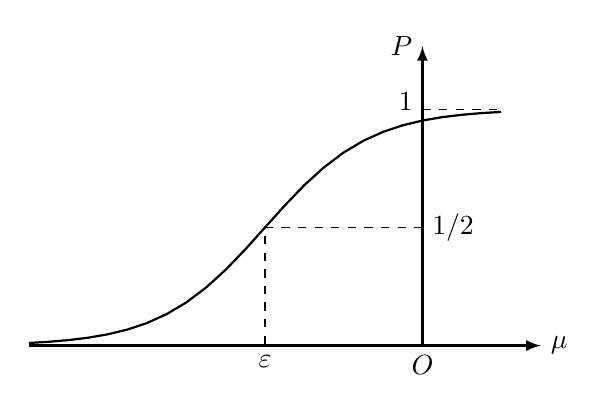
\begin{tikzpicture}
		\draw[thick,-latex](0,0)node[below]{$O$}--(0,3.8)node[left]{$\mathbb P$};
		\draw[thick,-latex](-5,0)--(1.5,0)node[right]{$\mu$};
		\draw[dashed](0,1.5)node[right]{$1/2$}--(-2,1.5)--(-2,0)node[below]{$\varepsilon$};
		\draw[dashed](0,3)--(1,3);
		\node at(0,3.1)[left]{1};
		\draw[thick,domain=-5:1]plot(\x,{3/(1+exp((-2-\x)*1.5))});
	\end{tikzpicture}
	\captionof{figure}{吸附位占据几率}
\end{center}
因此
\[
	\mu=\varepsilon-\kB T\ln\kh{{\mathbb P}^{-1}-1}.
\]

\sectionstar{非平衡热力学}
\subsection*{输运现象}
热导中,热流密度
\[\vec j_q=-\kappa\,\nabla T.\]
其中$\kappa$为热导率。
	电导中,电流密度
\[\vec j_e=-\sigma\,\nabla\phi.\]
即Ohm定律,其中$\sigma$为电导率。
	扩散中,
\[\vec j_n=D\,\nabla n.\]

\subsection*{熵的产生}
熵流
\[\dv st=\pv st+\nabla\cdot\vec J_s\]
这样热流密度
\[\vec J_q=T\vec J_s=\vec J_u-\mu\vec J_n\]
非平衡热力学基本方程
\[\dv st=\sum\vec F_i\cdot\vec J_i.\]
其中$\vec F_i:=\nabla A_i$为驱动力。

\newcommand*{\hji}{\scalebox{.4}[1]{火}\hspace{-4.3pt}\scalebox{.4}[1]{火}\hspace{-1pt}\scalebox{.7}[1]{积}}

\subsection*{\hji}
\hji\footnote{笑死,这个字根本打不出来。}(entransy)是清华大学过增元院士等通过热电类比提出的一个新的概念。顾名思义,\hji 被定义为热能和温度的积(的一半)
\[G:=\frac12QT.\]
在过院士等人的著作《传热\hji 理论及其应用》中,\hji 有热势能的含义,并类比熵的英文entropy,将\hji 的英文称作entransy。在书中,作者基于能量守恒方程推导了平衡方程,并提出耗散和耗散热阻等概念。通过平衡方程建立了系统内部传热引起的耗散与边界换热温差、热流之间的关系,为传热过程和热系统的优化提供了新的方法。%\underline{并差点得了科技进步奖。}
感兴趣的同学春季学期可以选修\textit{新概念热学(New Thermology)}\footnote{某老师更愿意简称其为NT。}。

\fi